\chapter{Plasma}
A plasma is a quasi-neutral gas of charged and neutral particles which exhibits collective behaviour \cite{plasma-intro3}. In simple terms, quasi-neutrality means that the density of electrons $n_e$ and density of positively charged ions $n_i$ locally satisfy:
\begin{equation}
	n_e \simeq Zn_i
\end{equation}
\noindent where $Ze$ is the charge of one positively charged ion and $e$ is elementary charge \cite{plasma-intro}. 

The non-neutral particles in plasma are subject to electric and magnetic fields generated either by external sources or by neighbouring particles. The long-range nature of $1/r$ Coulomb potential ensures that macroscopic fields dominate over forces created by microscopic fluctuations \cite{plasma-intro}. To explain the collective behaviour properly, one can start by writing \textit{Vlasov equation} \cite{laser-plasma4}:
\begin{equation}
	\frac{\partial f_j}{\partial t} + \bm{v} \cdot \frac{\partial f_j}{\partial \bm{x}} + \frac{q_j}{m_j}\left(\bm{E} + \frac{\bm{v}\times\bm{B}}{c}\right)\cdot \frac{\partial f_j}{\partial \bm{v}} = 0
\end{equation}
\noindent where $f_j = f_j\left(\bm{x},\bm{v},t\right)$ is the phase space distribution function, which characterizes the location of the particles of species $j$ (electrons or ions) in phase space $\left(\bm{x},\bm{v}\right)$ (position, velocity) as a function of time. $q_j$ and $m_j$ are charge and mass of the species $j$ and $c$ is the speed of light \cite{laser-plasma4}.

After calculating the 0th and 1st moment of Vlasov equation (averaging through $\bm{v}$), we obtain the equation of continuity and force equations for the density $n_j = \int f_j\left(\bm{x},\bm{v},t\right)\mathrm{d}\bm{v}$ and mean velocity $\bm{u}_j$ defined by $n_j\bm{u}_j = \int \bm{v} f_j\left(\bm{x},\bm{v},t\right)\mathrm{d}\bm{v}$:
\begin{equation}
	\label{eq:continuity}
	\frac{\partial n_j}{\partial t} + \nabla\cdot\left(n_j \bm{u}_j\right) = 0
\end{equation}
\begin{equation}
	\label{eq:momentum}
	n_j \left(\frac{\partial \bm{u}_j}{\partial t} + \left(\bm{u}_j\cdot\nabla\right)\bm{u}_j\right) = \frac{n_j q_j}{m_j}\left(\bm{E} + \frac{\bm{u}_j\times\bm{B}}{\mathrm{c}}\right) - \frac{1}{m_j}\nabla p_j
\end{equation}
\noindent where $p_j$ is pressure and in case of negligible heat flow also the energy equation:
\begin{equation}
	\label{eq:energy}
	p_jn_j^{-\gamma} = \mathrm{const.}.
\end{equation}
\noindent where $\gamma = \left(2+N\right)/N$ and $N$ is the number of degrees of freedom. Equations \ref{eq:continuity}, \ref{eq:momentum} and \ref{eq:energy} together with the Maxwell equations are often referred to as \textit{two-fluid model of plasma} and describe wide range of plasma (collective) behaviour such as plasma waves or Debye shielding \cite{laser-plasma4}.

\section{Temperature of plasma}
\label{sec:temperature-intro}
In this thesis, we are studying so called \textit{hot electrons} produced by the interaction of short laser pulse of high intensity with plasma. All important details of the physical phenomena will be covered in later sections, but let us now look at what is meant by $hot$ and how the temperature of plasma is usually understood.

In a gas in the thermal equilibrium, particles can have all velocities usually with Maxwellian distribution (in three dimensions) \cite{plasma-intro3}:
\begin{equation}
	f(\bm{v}) = n\left(\frac{m}{2\pi \boltz}\right)^{3/2}\exp\left(-\frac{\frac{1}{2}m v^2}{\boltz T}\right)
\end{equation} 
\noindent where $v = \norm{\bm{v}}$, $\boltz$ is the Boltzmann constant and $T$ is temperature. The average kinetic energy $E_{av}$ is then \cite{plasma-intro3}:
\begin{equation}
	E_{av}=\frac{3}{2}\boltz T
\end{equation}
Because of this relation between $E_{av}$ and $T$, it is customary in plasma physics to give the temperature the same units as energy. If $\boltz T = 1 \, \mathrm{eV} = 1.6 \times 10^{-19}\, \mathrm{J}$, then \cite{plasma-intro3}:
\begin{equation}
	T = \frac{1.6 \times 10^{-19}}{1.38\times 10^{-23}}=11600
\end{equation}
\noindent From this it follows that the factor of the conversion is:
\begin{equation}
	1 \mathrm{eV} = 11600\,\mathrm{K}
\end{equation} 
The electrons and the ions can have different temperature \cite{plasma-intro3}. What is more, there can be multiple groups of electrons with different distributions, but we will describe this more deeply in one of the later sections.

\section{Ionization}
Any substance can become plasma with the sufficient increase of its temperature. The threshold can vary, but usually can be found in the order of 1 eV, because any neutral atom binds the outer electron with a binding energy in order of 1 eV \cite{laser-plasma1}. The second important factor for ionization is the density of the condensed matter.

\subsection*{Density of plasma}
The thermodynamic equilibrium condition for the fraction of electrons $n(\epsilon)$ with energy $\epsilon$ is then:
\begin{equation}
	n(\epsilon) \propto g(\epsilon)f(\epsilon)
\end{equation}
\noindent where $g(\epsilon)$ is the density of state and $f(\epsilon)$ is the Fermi-Dirac distribution (function of $T$). In the extreme situation of density close to that of a vacuum, found in interstellar space, there are many states for free electrons that escaped from bound state, and $g(\epsilon)$ is large for free state compared to bound states. For example, for hydrogen atom with given principal quantum number $n^*$ there are $2\left(n^{*}\right)^2$ bound states. This is after the assumption that electron with $n>n^*$ is easily de-trapped. This means that the density of bound states is very low compared to free states and it is for this reason that the interstellar space is assumed to be filled with plasma even though $T\approx0$~\cite{laser-plasma1}.

The examples of plasmas of different densities and temperatures found in the real world can be seen in the table \ref{tab:den-temp}.

\begin{table}[hb]
	\centering
	\begin{tabular}{lcc}
		\textbf{Type}		& \textbf{Electron density}			 			 	& \textbf{Electron temperature} \\ 
			 				& $n_\mathrm{e}$ $\left[\mathrm{(cm)}^{-3}\right]$  &  $T_\mathrm{e}$ $\left[\mathrm{eV}\right]$ \\ \hline
		Stars 				& $10^{26}$          	& $2 \times 10^3$       \\
		Laser fusion    	& $10^{25}$           	& $3 \times 10^3$       \\
		Magnetic fusion		& $10^{15}$ 			& $10^3$         		\\
		Laser-produced		& $10^{18}$ - $10^{24}$ & $10^2$ - $10^3$       \\
		Discharges			& $10^{12}$          	& $1$ - $10$         	\\
		Ionosphere		    & $10^6$            	& $1.0$         		\\
		Interstellar medium & $1$               	& $10^{-2}$         	\\ \hline
	\end{tabular}
	\caption{Densities and temperatures of various plasma types \cite{plasma-intro}.}
	
	\label{tab:den-temp}
\end{table}

\subsection*{Critical density}
Now consider a high frequency electric field $\bm{E} = \bm{E(x)}\exp\left(-i\omega t\right)$. The frequency $\omega$ is assumed to be greater than electron plasma frequency $\omega_{\mathrm{pe}}$ defined as $\omega_{\mathrm{pe}}^2=4\pi e^2 n_0/m$ with $n_0=Zn_{0i}$ being electron density. Maxwell equations give us:
\begin{equation}
	\nabla \times \bm{B} = -\frac{i\omega}{c}\epsilon\bm{E},
\end{equation}
where $\epsilon = 1 - \omega_{\mathrm{pe}}^2/\omega^2$ defines the dielectric function of the plasma \cite{laser-plasma4}. After further derivation using the other Maxwell equations and vector identities we can get:
\begin{equation}
	\nabla^2 \bm{B} + \frac{\omega^2}{c^2}\epsilon\bm{B} + \frac{1}{\epsilon}\nabla\epsilon \times \left(\nabla \times \bm{B}\right) = 0
\end{equation}
Assuming space dependency described by $\exp\left(i\bm{k}\cdot\bm{x}\right)$, the dispersion relation is then:
\begin{equation}
	\omega^2 = \omega_{\mathrm{pe}}^2 + k^2c^2.
\end{equation}
It is possible to show, that $k$ becomes imaginary for $\omega < \omega_{\mathrm{pe}}$. It can be interpreted the following way: electrons shield out the field of a light wave if $\omega < \omega_{\mathrm{pe}}$. Because of that, $\omega_{\mathrm{pe}}=\omega$ defines the maximum plasma density to which a light wave can penetrate - \textit{critical density}:
\begin{equation}
	n_{\mathrm{cr}} = \frac{\omega^2 m}{4 \pi e^2} = 1.1 \times 10^{21} / \lambda_\mu^2 \, \mathrm{cm}^{-3}, 
\end{equation}
where $\lambda_\mu$ is the wavelength of the light in microns in vacuum \cite{laser-plasma4}.

\subsection*{Ionization mechanisms}
There are several mechanisms which can be used to describe ionization. One can start with directly hitting the atoms with fast particles, but for that one would need a stream of such particles. More common way of ionization is achieved by electromagnetic radiation (photoionization) or even via electrical breakdown in strong electric fields \cite{plasma-intro}. For this thesis, the only relevant ionization is through electromagnetic radiation - in our case a laser.

Firstly, oscillating electromagnetic field makes free electrons oscillate as well and they can ionize other atoms via collisions. New free electrons freed by the collisions can then also hit other atoms an so on.

There are also non-collisional mechanisms of ionization. Imagine field of hydrogen atom at Bohr radius $a_\mathrm{B}$ - the most probable distance of electron from the atomic nucleus:
\begin{equation}
	a_\mathrm{B} = \frac{\hbar}{me^2} = 5.3 \times 10^{-9} \, \mathrm{ cm}
\end{equation}
\noindent where $\hbar$ is the reduced Planck constant, $m$ is the mass of an electron and $e$ is the elementary charge.
The electric field for hydrogen $E_{\mathrm{H}}$ is then:
\begin{equation}
	E_{\mathrm{H}} = \frac{e}{4\pi\epsilon_0 a_\mathrm{B}^2} \simeq 5.1 \times 10^{9} \, \mathrm{V.m}^{-1}.
\end{equation}
\noindent Then the \textit{atomic intensity} for hydrogen $I_{\mathrm{H}}$ is \cite{plasma-intro}:
\begin{equation}
	I_{\mathrm{H}} = \frac{\epsilon_0 c E_{\mathrm{H}}^2}{2} \simeq 3.51 \times 10^{16} \, \mathrm{W.cm}^{-2}
\end{equation}
\noindent where $\mathrm{c}$ is the speed of light in vacuum.

It is reasonable to think that to ionize the hydrogen atom one needs $I_\mathrm{L}>I_{\mathrm{H}}$, where $I_{\mathrm{L}}$ is the intensity of the laser. In reality, the ionization occurs already for smaller laser intensities due to so called \textit{multiphoton absorption} \cite{plasma-intro} and \textit{quantum tunnelling} \cite{laser-plasma1}. The first one can occur, because the electron can climb the virtual energy states one after another and it can get hit by next photon before it falls back to lower energy state \cite{laser-plasma1}. The calculation of these transitions is non-trivial, because one has to solve time-dependant Schroedinger equation. The reader can find deeper analysis in \cite{atoms-in-lasers}.

The tunnelling effect is as well a consequence of the external electric field. The superposition of the electric field which binds the electron to the atom and the strong electric field of the laser results in conditions that allow the electron escape the potential well even if the electron energy is not higher than the threshold energy for instant ionization. Let $V_H(r)= -\frac{C}{r}$ Coulomb potential of hydrogen nucleus, where $C = \frac{e^2}{4\pi\epsilon_0}$. The superposition with strong external field gives us:
\begin{equation}
	V_F = V_H(r) + eE_{\mathrm{ext}}(r)
\end{equation}
Let $E_{\mathrm{ext}}(r) = -10^{10}r\,\mathrm{V/m}$. The final potential $V_\mathrm{F}$ together with highlighted region of tunneling can be seen in figure \ref{fig:tunnelling}. 

\begin{figure}[h]
	\centering
	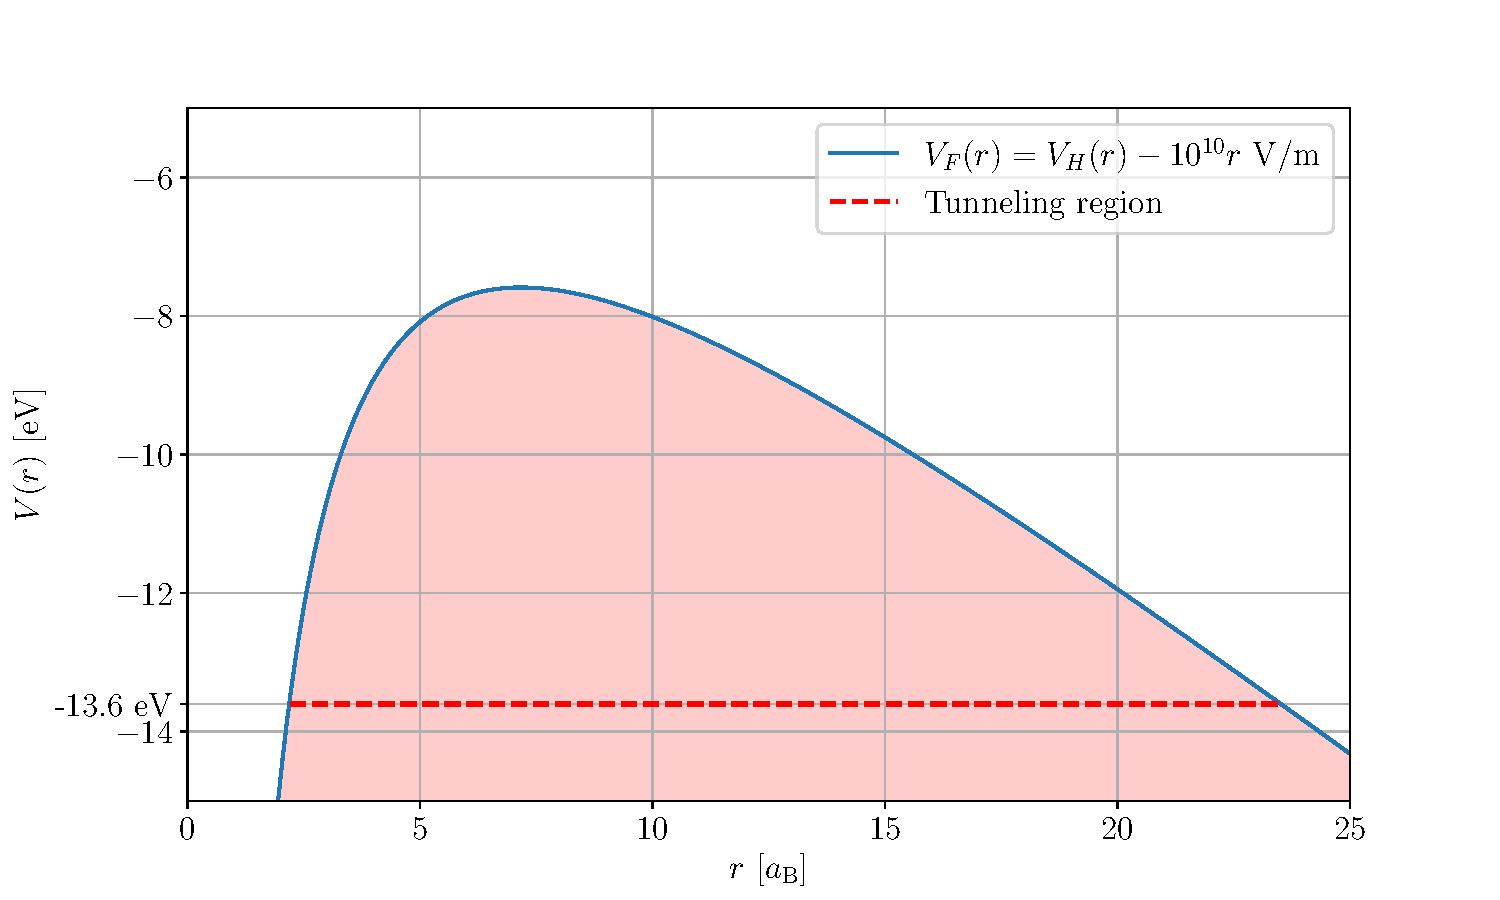
\includegraphics[width=0.8\textwidth]{figures/tunnelling}
	\caption{The potential of hydrogen atom modified by external field: $E_{\mathrm{ext}} = -10^{10}r\,\mathrm{V/m}$. $r$ is shown in radial coordinates with units of Bohr radius $\mathrm{a_B}$. Energy of ground state of electron in hydrogen atom $E_0 = 13.6 eV$ is highlighted.}
	\label{fig:tunnelling}
\end{figure}

The stronger is the external field, the shorter is the tunnelling distance for the electron to escape. The field can even be so strong that the potential barrier will have its peak below the ground state energy. In that case, the electron is instantly considered to be free \cite{laser-plasma1}. 

It is possible to estimate, which mechanism is more dominant cause of ionization by calculating so called \textit{Keldysh parameter} $\gamma_\mathrm{K} = \frac{\omega_0}{\omega_t}$, where $\omega_0$ is the frequency of the laser and $\omega_t = \frac{eE_{\mathrm{ext}}}{\sqrt{2mE_\mathrm{i}}}$, where $E_\mathrm{i}$ represents the energy the electron needs to receive to be ionized \cite{laser-plasma1}.

The ionization processes can be explored in greater depth, but the fundamental concepts have already been adequately outlined. Henceforth, we will assume the plasma being targeted by the laser is fully ionized and will focus on how it can absorb additional energy from the laser.

\section{Absorption of ultra-short, ultra-intense lasers}
Modern lasers can generate pulses with durations of only few femtoseconds and extremely high intensities (up to 
$10^{22}\,\mathrm{W.cm}^{-2}$) \cite{absorption2,ultra-laser}. The interaction of such pulses with dense plasma produces hot electrons \cite{laser-plasma5}. This interaction initiates several processes of energy transfer from the laser's electromagnetic field to the electrons. Let us examine the most significant of these processes.

\subsection*{Collisional absorption}
The principles of collisional absorption are similar to those of collisional ionization. In this process, an electron oscillates due to the influence of the laser field and transfers part of its kinetic energy to other ions through collisions. However, since the frequency of ion-electron collisions scales as $\nu_{ie} \propto E^{-3/2}$, this absorption mechanism is primarily significant for laser intensities below $10^{15}\,\mathrm{W.cm}^{-2}$ \cite{absorption1}. Given that this thesis focuses on intensities above this threshold, further discussion on collisional absorption is unnecessary.

\subsection*{Resonance absorption}
The first non-collisional absorption process we will describe is the \textit{resonance absorption}. This phenomenon can occur during the propagation of a p-polarized light wave through a density gradient. By p-polarized, we refer to a wave that is linearly polarized with its polarization vector lying in the plane of incidence. The complete analytical description is difficult, but after few simplifications it is possible to obtain reasonable idea of the principle \cite{laser-plasma6}. 

Laser light will reach density $n_t = n_{\mathrm{cr}}\cos^2\theta$ (from Snell's law \cite{absorption2}), where $\theta$ is the angle of incidence \cite{laser-plasma6}. Because of the p-polarization, some light energy will tunnel through the critical density and the electron plasma will be resonantly excited at frequency of the laser $\omega_0$. The resonant wave is then capable of accelerating electrons and is defined by:
\begin{equation}
	\label{eq:resonance}
	\frac{E_d}{\epsilon} = \frac{E_L}{\sqrt{2\pi\omega_0 L_n/c}}\phi\left(\tau\right)
\end{equation}
where $\epsilon$ is plasma dielectric function, $L_n$ is the density length scale and the parameter $\tau= \left(\omega_0 L_n/c\right)^{1/3}\sin\theta$ \cite{absorption2}. It can be approximated that $\phi\left(\tau\right) \propto \exp\left(-2\tau^3/3\right)$ \cite{laser-plasma6}.
Deeper derivation of te equation \ref{eq:resonance} can be found in \cite{laser-plasma6} starting on page 139.

The angle of optimum resonance absorption for exponential density profile $\theta_{opt}$ can then be estimated as a function of $L$:
\begin{equation}
	\theta_{opt}\left(L\right) = \arcsin\left(0.68(2\pi L)\right)
\end{equation}
where $L$ is normalized to the laser wavelength \cite{absorption1}.


\subsection*{Vacuum heating}
The second non-collisional absorption process (and no less important than the first one) is called \textit{Vacuum heating} or sometimes \textit{Brunel effect} or even \textit{“not-so-resonant” resonance absorption} \cite{brunel1987}. It was proposed by Mr.~Brunel in 1987 it was later confirmed by many experiments \cite{absorption2}.

Like before, p-polarized laser pulse is needed. At the angle of incidence $\theta$ the laser is hitting the target with steep density profile (a big gradient). A part of the pulse is refracted and a part is reflected. The incoming laser wave $\bm{E}_\mathrm{L}$ and reflected wave $\bm{E}_\mathrm{R}$ are in superposition at point of incidence $x=0$ and the resulting field has a perpendicular component with amplitude $E_0 =  2E_\mathrm{L}\sin\theta$, under approximation that $E_\mathrm{L}=E_\mathrm{R}$. Poisson's equation at the surface gives us \cite{absorption2}:
\begin{equation}
	\label{eq:poisson}
	\Delta E = -4\pi e\int_{x=-\Delta x}^{x=0}n \mathrm{d}x=4\pi e n \Delta x.
\end{equation}
The electrons are pulled out from plasma by that field according to the equation \ref{eq:poisson}. If $n=N/\left(A\Delta x\right)$ with $N/A$ being number of electrons pulled out into vacuum per unit area and if $\Delta E = E_0$, we get \cite{absorption2}:
\begin{equation}
	\frac{N}{A} = \frac{2E_0 \sin \theta}{4\pi e}.
\end{equation}
The energy absorbed $E_{\mathrm{abs}}$ by the electrons is then \cite{absorption2}:
\begin{equation}
	E_{\mathrm{abs}} = \frac{1}{2}N m_\mathrm{e} v_{\mathrm{e}}^2.
\end{equation}
After calculating the power absorbed by unit area and after substituting $v_0$ with \textit{quiver velocity} $v_{osc}$ defined by: $\frac{ v_{osc}}{c} = \frac{eE_0}{m_{\mathrm{e}}c\omega_0}$, we get the absorbed fraction of the power $f_{\mathrm{VH}} = I_{\mathrm{abs}}/I_0$ \cite{absorption2}:
\begin{equation}
	f_{\mathrm{VH}} = 8 \frac{v_{\mathrm{osc}}}{c}sin^3\theta
\end{equation}
Note that we made a simplification by letting $E_\mathrm{L}=E_\mathrm{R}$. Another option would be to directly write $E_0 =  \left(1+R^{1/2}\right)E_\mathrm{L}\sin\theta$, where $R$ is the reflectivity \cite{absorption1}. We also neglected that the electron in vacuum is very fast and therefore relativistic correction has to be made. It is possible to generally follow a more rigorous path found for example in \cite{laser-plasma5} and \cite{absorption1}. Then the formula for $f_{\mathrm{VH}}$ is expanded to:
\begin{equation}
	f_{\mathrm{VH}} = \frac{\eta}{2\pi}\frac{1}{a_0}\frac{sin\theta}{cos\theta}\left(1+R^{1/2}\right)\left\{\left[1+\left(1+R^{1/2}\right)^2a_0^2\sin^2\theta\right]^{1/2}-1\right\},
\end{equation}
where $\eta = 1.74$ and $a_0 = eE_\mathrm{L}/(m_\mathrm{e}\omega_0c)$.

\subsection*{$\bm{J}\times \bm{B}$ heating}
The last absorption mechanism we want to discuss is usually called $\bm{J}\times \bm{B}$ \textit{heating}. In the sections above, we discussed the heating of plasma due to electron motion in the direction of the oscillating $\bm{E}$ component of the laser beam. That is of course caused by the $e\bm{E}$ part of the Lorentz force. The other part - $\bm{j \times B}$ - can be neglected in non-relativistic cases. However, for laser intensities higher than $10^{17}\,\mathrm{W.cm}^{-2}$ it is not possible to explain all absorption using the classical limit and another consideration has to be made \cite{cai2006}.

Let $\phi$ and $\bm{A}$ be scalar and vector potential ($\bm{E} = \nabla \phi$ and $\bm{B} = \nabla \times \bm{A}$) satisfying Coulomb gauge $\nabla \cdot \bm{A} = 0$. Also, we can separate transverse and longitudinal part of electron momentum $\bm{p} = \bm{p}_\mathrm{t}+\bm{p}_\mathrm{l}$  Then the equations of motion for electron can be written as \cite{cai2006}:
\begin{equation}
	\frac{\partial \bm{p}_\mathrm{t}}{\partial t} = \frac{e}{c} \frac{\partial \bm{A}}{\partial t}
	\label{eq:jxb1}
\end{equation}
\begin{equation}
	\frac{\partial \bm{p}_\mathrm{l}}{\partial t} = e\nabla \phi - m_{\mathrm{e}}c^2\nabla (\gamma-1)
	\label{eq:jxb2}
\end{equation}
where $\gamma = \sqrt{1+\frac{p^2_\mathrm{osc}}{2m^2_\mathrm{e}c^2}}$ is the relativistic factor for linearly polarized light \cite{absorption2}. The second term of the equation \ref{eq:jxb2} is the relativistic ponderomotive force and we can write the ponderomotive potential $U_\mathrm{p}$ as:
\begin{equation}
	U_\mathrm{p} = m_{\mathrm{e}}c^2\nabla (1 -\gamma).
	\label{eq:ponderomotive-potential}
\end{equation}
After expanding $\gamma$ as a fourier series with frequency $\omega_0$:
\begin{equation}
	\gamma(z,t) = \gamma_0(z) + \gamma_1(z)\mathrm{e}^{i\omega_0t} + \gamma_2(z)\mathrm{e}^{i2\omega_0t} + ...
\end{equation}
we get $\gamma_1 = 0$ and $\gamma_2 \approx a_1^2/4$, where $a_1$ is defined with:
\begin{equation}
	\bm{a}(z,t) = e\bm{A}(z,t)/m_\mathrm{e}c^2 = \hat{\bm{x}}\frac{1}{2}\left[a_1(z)\mathrm{e}^{i\omega_0 t} + ...\right]
\end{equation}
where $\hat{\bm{x}}$ is a unit vector in the $x$ direction \cite{cai2006}. 

Thanks to the expansion, it is clear that there is a force with frequency $2\omega_0$ which will affect the electrons in longitudinal direction. One of the interpretations of this force can sound like this: 
Twice every laser period, streams of electrons are pushed into the the target \cite{cai2006}. This causes energy transfer to the rest of the plasma resulting in the production of fast electrons.

It is important to note, that at higher intensity, the electron density can rise as a consequence of the zero-frequency pondermotive force. The change in density can cause that the $2\omega_0$ resonance is not possible. The density is also dependent on the scale length of the target. For example for exponential density profile, the density decreases with the increase of scale length \cite{cai2006}. This means the $2\omega_0$ resonance is expected to play a greater role for bigger scale lengths. In other words, the initial plasma conditions need to be known to estimate the effects of $\bm{J}\times \bm{B}$ heating.

One last note regarding $\bm{J}\times \bm{B}$ heating. The relativistic factor $\gamma$ has a different form in a case of circularly polarized laser. That leads to suppressing this kind of electron heating altogether \cite{cai2006}.

\subsection*{Last words on absorption}
The three mentioned mechanisms are by no means exhaustive when it comes to laser absorption. They are the three most relevant in the context of this work. There are other physical contributing to heating up the plasma especially when the parameters of the experiment change \cite{absorption1}. We will now move on to motivating the thesis in greater detail.

\section{Motivation - X-ray emission}
Because hot electrons accelerated by ultra-intense ultra-short laser pulse can carry multi-keV energy, they can penetrate a solid behind the plasma, where by $K$-shell ionization they can generate X-rays \cite{reich2000}. The X-ray is consisting of spectral lines ($\mathrm{K}_\alpha$) and X-ray from Bremsstrahlung. The uniqueness of this method are the high energies of monochromatic photons within a short pulse synchronized with the laser pulse. The source is typically very small \cite{pfeifer2006}.

\begin{figure}[h]
	\centering
	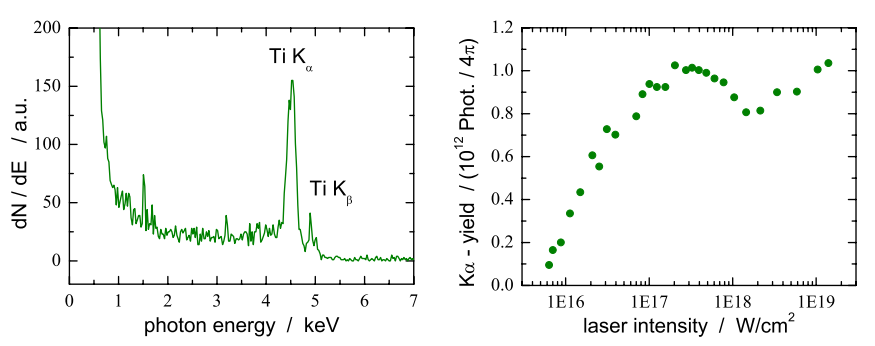
\includegraphics[width=0.95\textwidth]{figures/spectrum-ti}
	\caption{\textit{Left:} The spectrum of laser generated $\mathrm{K}_\alpha$ and $\mathrm{K}_\beta$ radiation of titanium. \textit{Right:} The scaling of $\mathrm{K}_\alpha$ - yield in relation to laser intensity. \cite{schwoerer2004}}
	\label{fig:ti-spectrum}
\end{figure}

Let us now briefly look into the origin $\mathrm{K}_\alpha$-line. In figure \ref{fig:ti-spectrum}, there is a spectrum of titanium for x-ray photon energies and how the $\mathrm{K}_\alpha$ - yield scales with the laser intensity. The generation of the $\mathrm{K}_\alpha$ radiation clearly depends on laser intensity and therefore in some sense also on hot electrons temperature. According to \cite{schwoerer2004}, the yield drops at the laser intensity around $10^{18}\,\mathrm{W.cm}^{-2}$ \textit{"because the interaction time with the atom decreases with higher electron velocity"}. The following rise in the yield is then attributed to the relativistic effect where the electric fields of the fast hot electrons are contracted and therefore have greater effect \cite{schwoerer2004}.

The total yield $N$ can be expressed analytically as \cite{reich2000}:
\begin{equation}
	N = \int n_\mathrm{hot} f_\mathrm{hot}(E) N_\mathrm{gen}(E) f_\mathrm{em}(E)\mathrm{d}E
	\label{eq:total-yield}
\end{equation}
where $N$ is the number of emitted photons, $n_\mathrm{hot}$ is the total number of hot electrons, and $f_\mathrm{hot}(E)$ is their energy distribution, $N_\mathrm{gen}(E)$ is the number of $\mathrm{K}_\alpha$ photons generated by an electron of incidence energy E, and $f_\mathrm{em}(E)$ is the fraction of these photons that escapes from the solid \cite{reich2000}. 

Having a reliable numerical model of $n_\mathrm{hot}$ and $f_\mathrm{hot}(E)$ from equation \ref{eq:total-yield} could allow us to optimize the $\mathrm{K}_\alpha$ yield based on the parameters of the laser and the plasma. Namely, the angle of incidence, the laser intensity and the plasma length scale. The research conducted by Reich et al. \cite{reich2000} could be followed up by examining a wider range of parameters beyond just laser intensity. This is crucial because, as shown by Cui et al. \cite{hot-electrons1}, the temperature function of the electrons has a complex and non-trivial shape. The complexity comes from the complex nature of the physical processes causing the electron heating.

In this thesis, we presents results from hundreds of PIC simulations while scanning through the mentioned parameters. Then we try to present and  defend a way of how the hot electron temperature can be modelled and how to make the model more precise. The implications with respect to previous works and to equation \ref{eq:total-yield} are discussed.

\section{PIC simulations}
As previously mentioned, we are using Particle-In-Cell (PIC) simulations to obtain the data necessary for our model. PIC codes have been under development since the advent of computers in the 1960s, and advancements in computer technology over the past 30 years have enabled us to run simulations on a much larger scale. One significant advantage of simulations is that they allow theoretical predictions to be verified in greater detail than is possible with real plasma experiments \cite{dawson1962}. To illustrate the progress made over the decades, let us mention, that in 1962 Dawson and Buneman simulated the motion of $1000$ plasma particles. Today, we can simulate the motion of more than $10^{10}$ particles \cite{tskhakaya2007}.

We are not developing our own simulation code. Instead, we are using code freely available for academic purposes, specifically the 2D simulation code EPOCH \cite{arber2015}. EPOCH has been widely used in numerous publications within the laser-plasma field and adequately meets our requirements. Below, we will present a brief overview of the key principles of the PIC method, upon which EPOCH is also based.

\subsection*{Macro-particles}
It is not possible to have as many particles in the simulation as in a real plasma, even in very small scales, because of the computational cost. That is why the simulations usually work with macro-particles which represent clouds of many real particles. These particles have finite sizes (as opposed to infinitesimal). In plasma simulations, it is possible to do this because of the collective behaviour \cite{fonseca2009} .

\subsection*{Computational cycle}
The simulation runs in a cycle. In each step, we solve for electromagnetic fields created by the charged particles. Then we evaluate the equations of motion for the particles, which are influenced by the Lorentz force \cite{birdsall1985}. The laser pulse is included as an external source of electromagnetic radiation at the boundary.

Typically, the finite-difference time-domain method (FDTD) is used for numerically solving Maxwell's equations, which fully describe the electromagnetic field. \textit{Finite-difference} means that the electric field $\bm{E}$ and magnetic field $\bm{B}$ are specified in the points of a grid - usually a \textit{Yee grid}. A comprehensive description of a Yee grid can be found in the original article by Yee \cite{yee1966}. The critical concept of a Yee grid is illustrated in figure \ref{fig:yee-grid}. - the magnetic field components are calculated in the center of the faces of an imaginary cube while the electric field components are calculated in the center of the edges. The cube represents one cell of the 3-dimensional grid. We can write derivatives of electric field \cite{arber2015}:
\begin{equation}
	\label{eq:num-der}
	\left(\frac{\partial E_y}{\partial x}\right)_{i+\frac{1}{2},j,k} = \frac{E_{y,i+1,j,k}-E_{y,i,j,k}}{\Delta x} 
\end{equation}

Note, that this numerical derivative in equation \ref{eq:num-der} is second order accurate at the cube point where we calculate $B_{z,i,j,k}$, because the formula is centered. Moreover, because of one of the Maxwell's equations, $\nabla \times \bm{E} = \frac{\partial \bm{B}}{\partial t}$, this derivative is exclusively used to calculate time-derivative of $B_{z,i,j,k}$. A similar relationship can be found when calculating all components of $\bm{B}$ from $\bm{E}$ and vice versa. Therefore, all used numerical derivatives are second order accurate \cite{arber2015}.

\begin{figure}[t]
	\centering
	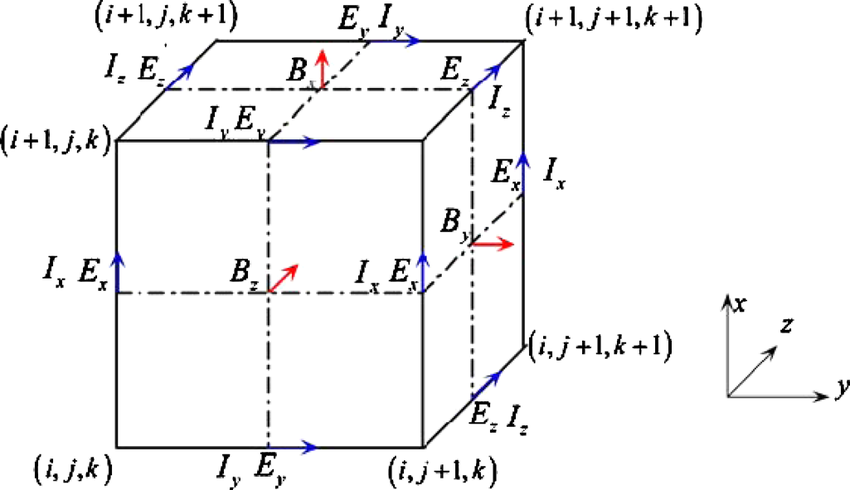
\includegraphics[width=0.6\textwidth]{figures/yee-grid}
	\caption{An illustration of a Yee grid \cite{wang2010}}.
	\label{fig:yee-grid}
\end{figure}

In EPOCH, as in other PIC codes, fields are updated at both the half time-step and full time-step. The first part - time-step from $n$ to $n+1/2$ - uses currents calculated at $n$:
\begin{equation}
	\bm{E}^{n+1/2} = \bm{E}^n + \frac{\Delta t}{2}\left(c^2 \nabla\times\bm{B}^n - \frac{\bm{J}^n}{\epsilon_0}\right)
\end{equation}
\begin{equation} 
	\bm{B}^{n+1/2} = \bm{B}^n - \frac{\Delta t}{2}\left(\nabla\times\bm{E}^{n+1/2} \right)
\end{equation}
where $\bm{J}$ is the current density and $\Delta t$ is a size of a full time-step \cite{arber2015}.

In the second step, with updated currents, we use the current extrapolated to step $n+1$:
\begin{equation} 
	\bm{B}^{n+1} = \bm{B}^{n+1/2} - \frac{\Delta t}{2}\left(\nabla\times\bm{E}^{n+1/2} \right)
\end{equation}
\begin{equation}
	\bm{E}^{n+1} = \bm{E}^{n+1/2} + \frac{\Delta t}{2}\left(c^2 \nabla\times\bm{B}^{n+1} - \frac{\bm{J}^{n+1}}{\epsilon_0}\right)
\end{equation}

The motion of particles and the resulting currents are consequences of these fields. Generally, the equations of motion are:
\begin{equation}
	\frac{\mathrm{d}\bm{x_l}}{\mathrm{d}t} = \bm{v_l} \text{   and   }  \frac{\mathrm{d}\bm{p_l}}{\mathrm{d}t} = \bm{F_l}
\end{equation}
where vectors $\bm{x_l}$,  $\bm{v_l}$  and $\bm{p_l}$ represent the position, velocity and momentum of the \textit{l}-th macro-particle. $\bm{F_l}=\bm{F_l}(t,\bm{x_l},\bm{v_l},\bm{E},\bm{B})$ is the force. Fields $\bm{E}$ and $\bm{B}$ are functions of the positions and velocities of the all charged particles \cite{tskhakaya2007}.
In this context, the right-hand side of the second equation represents the Lorentz force, and the time-step formula for the momentum is: \cite{arber2015}:
\begin{equation}
	\bm{p}^{~n+1}_{l} = \bm{p}^{~n}_l + q_l\Delta t \left[\bm{E}^{n+1/2}\left(\bm{x}_l^{~n+1/2}\right)+\bm{v_l}^{n+1/2}\times \bm{B}^{n+1/2}\left(\bm{x}_l^{~n+1/2}\right) \right] 
	\label{eq:mom-up}
\end{equation}
where $q_l$ is the charge of the $l$-th particle. The velocity can be calculated from the momentum using:
\begin{equation}
	\bm{v}_l = \frac{\bm{p}_l}{\gamma_l m_l}
\end{equation}
where $m_l$ is the mass of the particle and $\gamma_l = [p_l^2/(m_l^2 c^2)+1]^{1/2}$ is the corresponding gamma-factor \cite{arber2015}.

The particle position update is calculated from the velocity, but this is also done in multiple steps. First, we calculate movement of half time-step from the old velocity as we need it to update the momentum in equation \ref{eq:mom-up} \cite{arber2015}:
\begin{equation}
	\bm{x}^{~n+1/2}_{l} = \bm{x}^{~n}_l + \frac{\Delta t}{2} \bm{v}^{~n}_l  
\end{equation}
In similar way, we can then calculate $\bm{x}^{~n+1}_l$ and $\bm{x}^{~n+3/2}_l$ \cite{arber2015}, which are needed for calculating the currents.

The currents necessary for updating the fields can be calculated using methods such as the one presented by Esirkepov in \cite{esirkepov2001}. Modern approaches to calculating currents are generally based on solving the continuity equation:
\begin{equation}
	\frac{\partial\rho}{\partial t} + \nabla \cdot \bm{J} = 0
	\label{eq:conti}
\end{equation} 
where $\rho$ is the charge density and $\bm{J}$ is the electric current. This can be discretized as:
\begin{equation}
	\frac{\rho^{n+1}_{i+1/2,j+1/2,k+1/2}-\rho^{n}_{i+1/2,j+1/2,k+1/2}}{\Delta t} + \frac{J^{n+1/2}_{x,i+1,j+1/2,k+1/2}-J^{n+1/2}_{x,i,j+1/2,k+1/2}}{\Delta x} + \dots = 0.
\end{equation}

The charge density is calculated using \textit{form-factors} of macro-particles:

\begin{equation}
	\rho_{i,j,k} = \sum_{l}Q_l S_{i,j,k}(x_l,y_l,z_l)
\end{equation}
where $Q_l$ is the charge and $S_{i,j,k}(x_l,y_l,z_l)$ is the form-factor. During macro-particle motion, the total charge should remain constant, necessitating that the form-factors satisfy the condition :
\begin{equation}
	\sum_{i,j,k}S_{i,j,k}(x_l,y_l,z_l) = 1
\end{equation}
Since macro-particles in the simulation represent numerous real particles, a \textit{weight} is assigned to each macro-particle. Although the exact particle distribution within a macro-particle is unknown, a representative function, known as a \textit{shape function}, is chosen.\cite{arber2015}. 

Any function with a unit integral and compact support can be used as a shape function. An even distribution of particle in volume $\Delta x \times \Delta y \times \Delta z$ is referred to as the \textit{top hat} shape function. Using higher order shape functions are one of the improvements programmers were able to make thanks to more powerful computers. A higher order shape functions are for example triangular shape functions with volume of $2\Delta x \times 2\Delta y \times 2\Delta z$  . The weight is then calculated as a convolution of shape function with the 'top hat' function \cite{arber2015}.

Working with macro-particles instead of individual particles neglects some effects, particularly those effective over distances shorter than $\Delta x$. EPOCH uses a fully relativistic, energy-conserving binary collision model, which favors small-angle scattering to improve simulation behavior with a limited number of particles per cell. For our study involving laser intensities above $10^{10}$, collisions are not necessary. Other effects, such as ionization and quantum phenomena like photon emission and pair production, are often included when relevant, with detailed descriptions available in \cite{arber2015}.